\section{无粘浅水系统}

\textbf{无粘浅水方程组 (Inviscid Shallow Water Equations, SWEs)}是地球流体动力学的基本模型之一。
它将完整的三维流体问题简化为一个二维问题，但在水平面上完整地保留了科里奥利力和压力梯度力的影响。
因此，该模型能够描述诸如\textbf{表面重力波}、\textbf{Rossby波}等关键的大尺度现象。

在无粘浅水系统中，最核心的变量包括:

\begin{itemize}
    \item[$\freeheight(x, y, \timevar)$]: \textbf{自由面高度}，表示流体表面相对于某参考面的垂直高度。
    \item[$\bottomheight(x, y)$]: \textbf{底部地形高度}，即流体底部相对于参考面的高度。通常为不随时间变化的已知函数。
    \item[$\depth(x, y, \timevar)$]: \textbf{流体深度}，水体厚度定义为自由面与底部之间的距离: $\depth(x, y, \timevar) = \freeheight(x, y, \timevar) - \bottomheight(x, y)$。
\end{itemize}

另外，我们用添加下标 $h$ 的方式表示变量的水平方向分量。
例如水平方向的速度矢量:
\begin{equation*}
    \vel_h = (u, v, 0)
\end{equation*}

\subsection{物理模型}

我们将引入三个核心的、独立的假设来构建无粘浅水系统的物理模型。

\begin{enumerate}
    \item \textbf{无粘性 (Inviscid)}:
    忽略所有摩擦和耗散过程，即动量方程中 $\dissipation = 0$。

    \item \textbf{密度均匀且不可压缩 (正压性, Barotropic)}:
    我们假设流体是均质且不可压缩的，即密度 $\density$ 是一个常数。
    这排除了由温度或盐度差异引起的斜压效应 (Baroclinic Effects)。
    在这种情况下，流体的运动完全由力学因素驱动，是一个纯粹的动力学问题。

    因为密度均匀，连续性方程可以简化为不可压缩条件 $\nabla \cdot \vel = 0$，即流体体积守恒，无需考虑密度随时间和空间的变化。

    \item \textbf{浅水近似 (Shallow Water Approximation)}:
    忽略地球形状，我们假设流体的\textbf{水平尺度 $\hscale$ 远大于其垂直尺度 $\vscale$} ($\vscale \ll \hscale$)。
    即我们仅考虑一个非常扁平的几何结构。
\end{enumerate}

基于以上基本假设，我们可以推导出两个关键的推论:
\begin{itemize}
    \item \textbf{动力学推论: 静力平衡 (Hydrostatic Balance)}

    垂直方向的加速度 $\matderiv{w}$ 与重力 $\gravityconst$ 和垂直压力梯度力相比可以忽略不计。
    这使得垂直动量方程简化为\textbf{静力平衡方程}:
    \begin{equation}
        \pde{\pressure}{z} = -\density \gravityconst
        \label{eq:hydrostatic}
    \end{equation}

    这意味着垂直方向的压力分布完全由重力决定，从而极大地简化了压力场的结构。

    \begin{proofbox}[尺度分析]
        设水平速度、水平长度、垂直速度和垂直厚度的特征尺度分别为 $\hvel, \hscale, \vvel, \vscale$。
        \begin{itemize}
            \item \textbf{估算垂直速度 $\vvel$}: 根据不可压缩条件 $\nabla \cdot \vel = 0$，我们有 $\frac{\vvel}{\vscale} \sim \frac{\hvel}{\hscale}$，因此 $\vvel \sim \hvel \frac{\vscale}{\hscale}$。由于 $\vscale \ll \hscale$，这意味着 $\vvel \ll \hvel$。

            \item \textbf{估算垂直加速度}: $\matderiv{w}$ 的尺度约为 $\frac{\hvel^2 \vscale}{\hscale^2}$。

            \item \textbf{量级比较}: 以大尺度天气系统为例，典型参数如下:
            \begin{itemize}
                \item 水平速度 $\hvel \sim 50\,\mathrm{m/s}$: 对流层内强风带或急流的典型风速。
                \item 垂直厚度 $\vscale \sim 10\,\mathrm{km}$: 对流层的高度范围。
                \item 水平长度 $\hscale \sim 1000\,\mathrm{km}$: 中纬度气旋、锋面等天气系统的水平尺度。
            \end{itemize}

            代入上述数值，可得:
            \begin{equation*}
                \matderiv{w} \sim \frac{\hvel^2 \vscale}{\hscale^2} = \frac{50^2 \times 10^4}{(10^6)^2} = 2.5 \times 10^{-5}\,\mathrm{m/s^2} \quad \ll \quad \gravityconst \sim 10\,\mathrm{m/s^2}
            \end{equation*}

            因此，在浅水近似下我们可以合理地忽略垂直加速度。
        \end{itemize}
    \end{proofbox}

    \item \textbf{运动学推论: 柱状运动 (Columnar Motion)}

    由于流体密度均匀且满足静力平衡，$\nabla_h \pressure = \nabla_h (\int_z^\freeheight \density \gravityconst \dd{z^\prime}) = \density \gravityconst \nabla_h \freeheight$。
    这说明水平压力梯度 $\nabla_h \pressure$ 不随深度 $z$ 变化，表明驱动水平运动的压力梯度力在整个流体柱中是均匀的。因此，如果流体初始的水平速度不随深度变化，那么在后续的运动中它将整体移动，保持垂直柱状结构:
    \begin{equation}
        \pde{\vel_h}{z} = 0
        \label{eq:columnar_motion}
    \end{equation}
\end{itemize}

\subsection{基本方程组的简化}

现在，我们将上述假设与推论应用于原始的基本方程组，以推导出无粘浅水情况下的方程组。

\subsubsection{动量方程的简化}

\begin{enumerate}
    \item \textbf{压力场结构}:
    将静力平衡方程 \eqref{eq:hydrostatic} 从任意深度 $z$ 积分到流体的自由表面 $z= \freeheight(x, y, \timevar)$:
    \begin{equation*}
        \int_z^\freeheight \pde{\pressure}{z^\prime} \dd{z^\prime} = \int_z^\freeheight -\density \gravityconst \dd{z^\prime}
    \end{equation*}

    假设自由表面的压力为常数 $\pressure_s$，我们得到任意深度的压力:
    \begin{equation}
        \pressure(x, y, z, \timevar) = \pressure_s + \density \gravityconst (\freeheight(x, y, \timevar) - z)
        \label{eq:swe_pressure_field}
    \end{equation}

    该结果表明\textbf{三维压力场完全由二维的自由表面高度 $\freeheight$ 决定}。

    \item \textbf{压力梯度力}:
对压力场 \eqref{eq:swe_pressure_field} 求水平梯度:
    \begin{equation*}
        \nabla_h \pressure = \nabla_h (\pressure_s + \density \gravityconst \freeheight - \density \gravityconst z) = \density \gravityconst \nabla_h \freeheight
    \end{equation*}

    构造得到压力梯度算子 $\opP$ 的水平分量:
    \begin{equation*}
        \left(\opP\right)_h = -\frac{1}{\density}\nabla_h \pressure = -\frac{1}{\density}(\density \gravityconst \nabla_h \freeheight) = -\gravityconst \nabla_h \freeheight
    \end{equation*}

    \item \textbf{水平动量方程}:
    将简化后的压力梯度力代入原始动量方程 \eqref{eq:momentum_lagrangian}，并应用无粘 ($\dissipation = 0$)和柱状运动 ($\vel_h = \vel_h(x, y, \timevar)$) 的假设，我们得到:
    \begin{equation}
        \matderiv{\vel_h} = -\coriolis \kvec \times \vel_h - \gravityconst \nabla_h \freeheight
        \label{eq:momentum_shallow}
    \end{equation}
\end{enumerate}

\subsubsection{连续性方程的简化}

\begin{enumerate}
    \item \textbf{运动学边界条件}:
    流体质点不会穿过自由表面和底部。
    因此我们有边界条件:
    \begin{itemize}
        \item 在自由表面 $z = \freeheight(x, y, \timevar)$ 处: $w(\freeheight) = \matderiv{\freeheight} = \pde{\freeheight}{\timevar} + \vel_h \cdot \nabla_h \freeheight$
        \item 在底部 $z = \bottomheight(x, y)$ 处: $w(\bottomheight) = \matderiv{\bottomheight} = \pde{\bottomheight}{\timevar} + \vel_h \cdot \nabla_h \bottomheight$
    \end{itemize}

    假定底部地形不随时间变化，则 $\pde{\bottomheight}{\timevar} = 0$。

    \item \textbf{垂向积分}:
    改写不可压缩条件 $\nabla \cdot \vel = 0$ 为 $\pde{w}{z} = -(\nabla_h \cdot \vel_h)$。
    然后从流体底部 $z = \bottomheight(x, y)$ 积分到自由表面 $z = \freeheight(x, y, \timevar)$:
    \begin{equation*}
        \int_{\bottomheight}^\freeheight \pde{w}{z} \dd{z} = \int_{\bottomheight}^\freeheight -(\nabla_h \cdot \vel_h) \dd{z}
    \end{equation*}

    由于柱状运动假设 ($\vel_h$ 不依赖于 $z$):
    \begin{equation*}
        w(\freeheight) - w(\bottomheight) = -(\nabla_h \cdot \vel_h) (\freeheight - \bottomheight)
    \end{equation*}

    \item \textbf{厚度方程}:
    将边界条件代入上式:
    \begin{align*}
        (\pde{\freeheight}{\timevar} + \vel_h \cdot \nabla_h \freeheight) - (\vel_h \cdot \nabla_h \bottomheight) &= -(\nabla_h \cdot \vel_h) \depth \\
        \pde{\freeheight}{\timevar} + \vel_h \cdot \nabla_h \depth + \depth(\nabla_h \cdot \vel_h) &= 0
    \end{align*}

    由于 $\pde{\bottomheight}{\timevar} = 0$，$\depth = \freeheight - \bottomheight$，于是 $\pde{\depth}{\timevar} = \pde{\freeheight}{\timevar}$，即得:
    \begin{itemize}
        \item \textbf{欧拉形式}:
        \begin{equation}
            \pde{\depth}{\timevar} + \nabla_h \cdot (\depth \vel_h) = 0
            \label{eq:thickness_eulerian}
        \end{equation}

        \item \textbf{拉格朗日形式}:
        \begin{equation}
            \matderiv{\depth} + \depth (\nabla_h \cdot \vel_h) = 0
            \label{eq:thickness_lagrangian}
        \end{equation}
    \end{itemize}

    该方程描述了\textbf{流体柱的体积守恒}，也被称为\textbf{厚度方程}。
    这表明水平辐散 ($\nabla_h \cdot \vel_h > 0$) 将导致流体柱垂直下沉，而水平辐合 ($\nabla_h \cdot \vel_h < 0$) 将导致流体柱垂直上升。
\end{enumerate}

\subsection{守恒性质 (Conservation Laws)}

\subsubsection{流体柱内相对位置的守恒}

在无粘浅水系统的柱状运动假设下，\textbf{一个流体质点在垂直流体柱中的相对位置是守恒的}:
\begin{equation}
    \matderiv{} \left(\frac{z - \bottomheight}{\depth}\right) \equiv 0
    \label{eq:relative_position_conservation}
\end{equation}

\begin{proofbox}
    由柱状运动假设，水平速度 $\vel_h$ 不依赖于 $z$，对不可压缩条件 $\pde{w}{z} = -(\nabla_h \cdot \vel_h)$ 积分:
    \begin{equation*}
        w(z) - w(\bottomheight) = -(\nabla_h \cdot \vel_h)(z - \bottomheight)
    \end{equation*}

    代入边界条件，并利用厚度方程 \eqref{eq:thickness_lagrangian}:
    \begin{equation*}
        \matderiv{(z - \bottomheight)} = w(z) - w(\bottomheight) = (z - \bottomheight) (-\nabla_h \cdot \vel_h) = \frac{z - \bottomheight}{\depth} \matderiv{\depth}
    \end{equation*}

    整理得:
    \begin{equation*}
        0 = \frac{1}{\depth^2} \left(\depth \matderiv{(z - \bottomheight)} - (z - \bottomheight) \matderiv{\depth}\right) = \matderiv{} \left(\frac{z - \bottomheight}{\depth}\right)
    \end{equation*}
\end{proofbox}

\subsubsection{位涡守恒 (Potential Vorticity Conservation)}

\textbf{位涡 (Potential Vorticity, PV)}是描述流体涡旋运动的一个重要物理量。
在无粘浅水系统中，它将流体的绝对涡度 (自身旋转与地球旋转之和) 与流体柱的厚度联系了起来。

首先，我们定义相关概念:
\begin{itemize}
    \item \textbf{相对涡度 (Relative Vorticity)} $\relvort$:
    速度场 $\vel_h$ 的水平旋度，描述了流体相对于地球的局地旋转。
    \begin{equation}
        \relvort = \kvec \cdot (\nabla_h \times \vel_h) = \pde{v}{x} - \pde{u}{y}
        \label{eq:def_relative_vorticity}
    \end{equation}

    \item \textbf{绝对涡度 (Absolute Vorticity)} $\absvort$:
    相对涡度与行星涡度 (即科里奥利参数 $\coriolis$) 之和。
    \begin{equation}
        \absvort = \relvort + \coriolis
        \label{eq:def_absolute_vorticity}
    \end{equation}

    \item \textbf{位涡 (Potential Vorticity)} $\pv$:
    绝对涡度 $\absvort$ 与流体柱厚度 $\depth$ 的比值。
    \begin{equation}
        \pv = \frac{\relvort + \coriolis}{\depth}
        \label{eq:def_potential_vorticity}
    \end{equation}
\end{itemize}

\textbf{在无粘浅水系统中，一个流体质点所携带的位涡是一个守恒量。}
\begin{equation}
    \matderiv{\pv} = \matderiv{}\left(\frac{\relvort + \coriolis}{\depth}\right) \equiv 0
    \label{eq:pv_conservation}
\end{equation}

\begin{proofbox}
    首先，对水平动量方程 \eqref{eq:momentum_shallow} 作用水平旋度算子 $\kvec \cdot (\nabla_h \times \cdot)$，得到涡度方程:
    \begin{equation*}
        \underbrace{\kvec \cdot \left(\nabla_h \times \matderiv{\vel_h}\right)}_{\text{涡度变化}} = \underbrace{-\kvec \cdot \left(\nabla_h \times (\coriolis \kvec \times \vel_h)\right)}_{\text{科里奥利项}} \underbrace{-\gravityconst \kvec \cdot (\nabla_h \times \nabla_h \eta)}_{\text{压力梯度项}}
    \end{equation*}

    \begin{enumerate}
        \item \textbf{涡度变化}: 跟随流体运动的涡度变化，等于涡度自身的物质导数，加上由于流体柱被拉伸或压缩 (辐散项 $\nabla_h \cdot \vel_h$) 而导致的涡度变化 (涡旋拉伸效应，详见\eqref{eq:vortex_stretching_proof})。
        \begin{equation}
            \kvec \cdot \left(\nabla_h \times \matderiv{\vel_h}\right) = \matderiv{\relvort} + \relvort (\nabla_h \cdot \vel_h)
            \label{eq:vortex_stretching}
        \end{equation}

        \item \textbf{科里奥利项}: 科里奥利力的水平旋度体现于行星涡度随纬度与辐散项的变化。
        \footnote{使用矢量恒等式 $\nabla \times (\ivec{f} \times \ivec{g}) = (\ivec{g} \cdot \nabla)\ivec{f} - (\ivec{f} \cdot \nabla)\ivec{g} + \ivec{f}(\nabla \cdot \ivec{g}) - \ivec{g}(\nabla \cdot \ivec{f})$。}
        \begin{equation*}
            -\kvec \cdot \left(\nabla_h \times (\coriolis \kvec \times \vel_h)\right) = -\coriolis(\nabla_h \cdot \vel_h) - \vel_h \cdot \nabla_h \coriolis = -\coriolis(\nabla_h \cdot \vel_h) - \matderiv{\coriolis}
        \end{equation*}

        \item \textbf{压力梯度项}: 标量场梯度的旋度恒为零，故 $\nabla_h \times \nabla_h \eta = 0$。
    \end{enumerate}

    整理结果，我们得到了\textbf{绝对涡度方程}:
    \begin{equation}
        \matderiv{(\relvort + \coriolis)} + (\relvort + \coriolis) (\nabla_h \cdot \vel_h) = 0
        \label{eq:absolute_vorticity_equation}
    \end{equation}
    利用厚度方程 \eqref{eq:thickness_lagrangian}:
    \begin{equation*}
        0 = \frac{1}{\depth} \left(\matderiv{(\relvort + \coriolis)} - \frac{\relvort + \coriolis}{\depth} \matderiv{\depth}\right) = \matderiv{}\left(\frac{\relvort + \coriolis}{\depth}\right) = \matderiv{\pv}
    \end{equation*}
\end{proofbox}

\subsubsection{背风槽 (Lee Trough)}

背风槽是指在高大山脉背风侧 (下风方向) 形成的低压槽状气压场结构，是中纬度大气环流中常见的重要天气系统。

如图 \ref{fig:lee_trough}，我们以落基山脉为例，详细分析背风槽的动力学形成机制。
落基山脉横亘于北美大陆西部，是西风带气流的重要障碍。
气流自西向东遇到山脉时，在迎风坡 (西侧) 被迫抬升，流体柱厚度 $\depth$ 随地形升高而减小。
根据无粘浅水系统的\textbf{位涡守恒} ($\matderiv{\pv} = \matderiv{}\left(\frac{\relvort + \coriolis}{\depth}\right) = 0$)，当流体柱厚度 $\depth$ 减小时，绝对涡度 $\relvort + \coriolis$ 也必须减小以保持 $\pv$ 不变;气流越过山脉后，背风坡 (东侧) 地势迅速降低，$\depth$ 增大，此时绝对涡度 $\relvort + \coriolis$ 必须增大。

假定初始时气流的相对涡度 $\relvort = 0$，行星涡度 $\coriolis$ 在中纬度变化较小，绝对涡度的变化主要通过 $\relvort$ 实现。
气流上山时，$\depth$ 减小，$\relvort$ 变为负值 (反气旋性)，气流轨迹向南偏;下山时，$\depth$ 增大，$\relvort$ 增大，反气旋性减弱甚至转为气旋性，气流轨迹向北偏。

\begin{figure}[H]
    \centering
    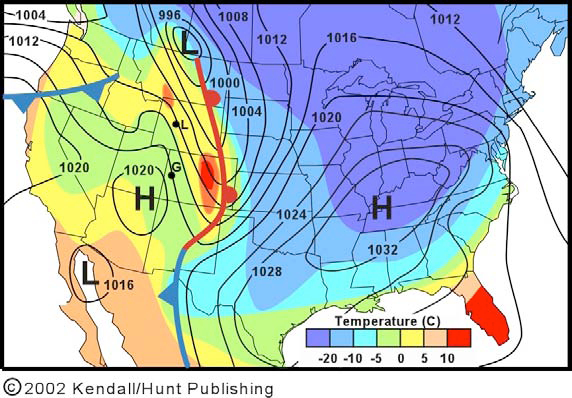
\includegraphics[width=1.00\textwidth]{assets/lee_trough_diagram.png}
    \caption{在落基山脉背风侧形成的低压槽}
    \label{fig:lee_trough}
\end{figure}

如果山脉对称，理论上上山和下山过程的相对涡度变化可抵消，气流在山脚的相对涡度恢复为零。
但实际上，由于气流过山的全过程均为反气旋式路径，到达山脚时气流已偏南，科里奥利参数$\coriolis$偏小，相对涡度需进一步增大 (下山时增幅大于上山时减幅)，在山脚可出现正涡度路径，气流轨迹向北弯曲。
当气流返回初始纬度时，相对涡度又恢复为零，但由于惯性，气流会继续向北，科里奥利参数$\coriolis$增大，相对涡度减小，轨迹再向南，从而形成准周期性的南北摆动。
如此，在背风坡将形成一系列槽脊，但因摩擦作用，只有第一个槽最明显，称为背风槽。

\subsection{小振幅波动理论 (Small Amplitude Wave Theory)}

波动是振动在空间中的传播，具有时空双重周期性。
任一波动可以视为不同频率和振幅的简谐波之叠加。
我们可以简洁地使用\textbf{复指数函数}来表示简谐波:
\begin{equation}
    \wavefunc(\pos, \timevar) = \amplitude \complexexp{(\wavenumber \cdot \pos - \frequency \timevar + \phase_0)} = \complexamp{\wavefunc} \complexexp{(\wavenumber \cdot \pos - \frequency \timevar)} = \complexamp{\wavefunc} \complexexp{\wavenumber \cdot (\pos - \wavespeed \timevar)}
    \label{eq:harmonic_wave}
\end{equation}

其中，$\amplitude$ 是振幅，$\wavenumber = (k, l, m)$ 是波数，$\frequency$ 是角频率，$\phase_0$ 是初始相位。
另外，我们还定义了复振幅 $\complexamp{\wavefunc} = \amplitude \complexexp{\phase_0}$ 和相速度 $\wavespeed = \frac{\frequency}{\wavenumber}$。
记周期为 $\period = \frac{2\pi}{\frequency}$，波长为 $\wavelength = \frac{2\pi}{\wavenumber}$。

在地球流体中，波动是能量和动量传播的主要方式。
然而，对于完整的流体方程组，通常难以求得解析解。
为研究波动的基本性质，我们采用\textbf{小振幅近似}，将方程线性化，从而分离出不同类型的波动解。

\subsubsection{线性化方法 (Linearization Method)}

线性化的核心思想是将流场物理量分解为\textbf{基本态} (背景场) 与\textbf{微小扰动}之和。
设任一物理量 $\wavefunc$ 可表示为:
\begin{equation}
    \wavefunc = \wavefunc_0 + \wavefunc^\prime
    \label{eq:wavefunc_decomposition}
\end{equation}

其中，$\wavefunc_0$ 是已知的基本态，满足原方程和定解条件。
在设置 $\wavefunc_0$ 时，通常可以考虑距平 (Anomaly) 或空间平均 (纬圈平均、垂直廓线) 。
我们认为小扰动量 $\wavefunc^\prime$ 相对于基本态 $\wavefunc_0$ 足够小，即 $\norm{\wavefunc^\prime} \ll \norm{\wavefunc_0}$。
在此前提下，我们可以将 $\wavefunc^\prime$ 及其导数的二阶乘积项可以略去 (忽略二阶小量) 。

将此表达式代入原始方程，利用基本态满足定常解条件，并忽略所有二阶小量 (两个或以上扰动量的乘积) ，即可得到描述扰动演化的线性方程组。

现在，将该方法应用于无粘浅水方程组。
考虑最简单的基本态: 静止且深度均匀的流体层，即 $\vel_0 = 0$，$\depth_0 = \text{const}$。
扰动表现为微弱的速度场 $\vel_h^\prime$ 和深度变化 $\depth^\prime$:
\begin{equation*}
    \vel_h = \vel_h^\prime, \quad \depth = \depth_0 + \depth^\prime
\end{equation*}

将它们代入水平动量方程 \eqref{eq:momentum_shallow} 和厚度方程 \eqref{eq:thickness_eulerian}:
\begin{align*}
    \pde{\vel_h^\prime}{\timevar} + (\vel_h^\prime \cdot \nabla_h) \vel_h^\prime &= - \coriolis \kvec \times \vel_h^\prime - \gravityconst \nabla_h \freeheight \\
    \pde{(\depth_0 + \depth^\prime)}{\timevar} + \nabla_h \cdot ((\depth_0 + \depth^\prime)\vel_h^\prime) &= 0
\end{align*}

其中，由于底部地形平坦，$\bottomheight$ 为常数，$\nabla_h \freeheight = \nabla_h \depth = \nabla_h \depth^\prime$。
定义\textbf{重力势}:
\begin{equation}
    \gravpotential^\prime = \gravityconst \depth^\prime \label{eq:gravpotential}
\end{equation}

定义特征速度: $C_0 = \sqrt{\gravityconst \depth_0}$。
忽略二阶小量，我们得到\textbf{线性化的无粘浅水方程组}:
\begin{align}
    \pde{\vel_h^\prime}{\timevar} &= -\coriolis \kvec \times \vel_h^\prime - \nabla_h \gravpotential^\prime \label{eq:linear_swe_momentum} \\
    \pde{\gravpotential^\prime}{\timevar} + C_0^2 (\nabla_h \cdot \vel_h^\prime) &= 0 \label{eq:linear_swe_thickness}
\end{align}

\subsubsection{表面重力波 (Surface Gravity Waves)}

\textbf{表面重力波}是上下边界的地球流体受到垂直扰动，偏离平衡位置，在重力作用下形成的波动。
我们暂时忽略地球自转的影响，即设科里奥利参数 $\coriolis = 0$。
此时，方程组 \eqref{eq:linear_swe_momentum}，\eqref{eq:linear_swe_thickness} 进一步简化为:
\begin{equation*}
    \pde{\vel_h^\prime}{\timevar} = -\nabla_h \gravpotential^\prime, \quad \pde{\gravpotential^\prime}{\timevar} + C_0^2 (\nabla_h \cdot \vel_h^\prime) = 0
\end{equation*}

注意到，此即为波动方程的一般形式。
定义\textbf{重力外波算子}: $\opG = \pde[2]{}{\timevar} - C_0^2 \nabla_h^2$，有:
\begin{equation}
    \opG{\vel_h^\prime} = 0, \quad \opG{\gravpotential^\prime} = 0
    \label{eq:wave_equation_gravity}
\end{equation}

波动方程的解为:
\begin{equation}
    (\vel_h^\prime, \gravpotential^\prime) = (\complexamp{\vel_h^\prime}, \complexamp{\gravpotential^\prime}) \complexexp{(\kvec_h \cdot \pos_h - \frequency \timevar)} \label{eq:wave_solution_gravity}
\end{equation}

将解代入 \eqref{eq:wave_equation_gravity}，得到频散关系 (Dispersion Relation):
\begin{equation}
    \frequency^2 = C_0^2 \norm{\wavenumber_h}^2
    \label{eq:dispersion_relation_gravity}
\end{equation}

因此，特征速度即为表面重力波的波速:
\begin{equation}
    \norm{\wavespeed} = \norm{\frac{\frequency}{\wavenumber_h}} = C_0 = \sqrt{\gravityconst \depth_0}
    \label{eq:gravity_wave_speed}
\end{equation}

这表明表面重力波具有\textbf{无频散性 (Non-dispersive)}，其传播速度 $\norm{\wavespeed}$ 仅由流体平均深度 $\depth_0$ 决定，而与波长或频率无关。
这意味着对于表面重力波，所有波长的波都以相同的速度传播，因此一个由多列波叠加而成的波包在传播过程中不会变形。

在垂直方向上对不可压缩条件 $\pde{w}{z} = -(\nabla_h \cdot \vel_h)$ 积分，考虑底部边界条件 $w(\bottomheight) = 0$，得到垂直方向上的速度:
\begin{equation}
    w = -z (\nabla_h \cdot \vel_h)
    \label{eq:vertical_velocity_shallow}
\end{equation}

可以看出，表面重力波只在水平方向上传播。
它发生在边界面上，距离扰动边界越远，波动越不明显，振幅在自由面上的速度最大。

\begin{insightbox}[表面重力波的物理图景]
    表面重力波的产生源于流体自由表面对平衡位置的偏离。
    当流体表面受到扰动而产生起伏时，高处的流体在重力作用下向下运动，低处则相应抬升。
    由于流体的不可压缩性，表面的下沉必然伴随着水平方向的外流 (辐散) ，而表面的抬升则伴随着水平方向的内流 (辐合) 。
    这种水平辐散与辐合在垂直方向的积分效应，通过连续性方程与表面高度变化率联系起来，构成了波动传播的动力学基础。

    在这一过程中，重力是唯一的恢复力——它试图将偏离平衡位置的流体拉回，但流体的惯性使其越过平衡位置，从而形成持续的振荡。
    这种振荡在空间中的传播，就是我们观测到的表面重力波。
\end{insightbox}

在地球系统中，表面重力波是典型的\textbf{快波 (Fast Wave)}。
取典型深度 $\depth_0 = 4000\,\mathrm{m}$，可得: $\norm{\wavespeed} \approx 200\,\mathrm{m/s} = 720\,\mathrm{km/h}$。
这一速度远大于流体本身的平流速度，因此表面重力波能够快速调整流场，使系统趋向平衡态。

\subsubsection{Rossby波}

\textbf{Rossby波} (罗斯贝波，或称大气长波、行星波) 是一种大尺度波动，其恢复力来自于\textbf{科里奥利参数随纬度的变化}。
Rossby波常出现在大气对流层中上层，波长可达数千公里，沿纬圈呈3\textasciitilde5个波，波速接近风速。
Rossby波很大程度上影响天气变化，特别是在对流较弱时 (如冬季) 。
因为Rossby波的存在，天气过程往往存在着5-7天或7-10天的准周期。

对于大尺度运动 (Rossby数 $\ro = \frac{\hvel}{\coriolis_0 \hscale} \ll 1$)，可近似认为水平速度场无辐散: $\nabla_h \cdot \vel_h^\prime \approx 0$。

为定量描述科里奥利参数随纬度的变化，我们定义Rossby参数:
\begin{equation}
    \rossby = \ode{\coriolis}{y}
    \label{eq:rossby_parameter}
\end{equation}

为简化分析，我们引入\textbf{ $\beta$ 平面近似 ($\beta$-plane Approximation)}。
我们将科里奥利参数 $\coriolis$ 在某个中心纬度 $\latitude_0$ 附近作Taylor展开，然后仅保留至线性项:
\begin{equation}
    \coriolis(y) = \coriolis(\latitude_0) + \left.\ode{\coriolis}{\latitude}\right|_{\latitude_0} (\latitude - \latitude_0) + \dots \approx \coriolis_0 + \rossby_0 y
    \label{eq:beta_plane}
\end{equation}

其中，$y$ 是从中心纬度向北的局地笛卡尔坐标，$\coriolis_0 = 2\norm{\rotationvec} \sin\latitude_0$。

设 $\earthradius$ 为地球半径，Rossby参数为:
\begin{equation}
    \rossby_0 = \left.\ode{\coriolis}{y}\right|_{y = 0} = \frac{2 \norm{\rotationvec} \cos\latitude_0}{\earthradius}
    \label{eq:rossby_parameter_value}
\end{equation}

在赤道附近，Rossby参数的值为 $\rossby_0 = 2 \times \frac{7.292 \times 10^{-5}}{6.371 \times 10^6} = 2.289 \times 10^{-11}\,\mathrm{m^{-1} s^{-1}}$。

为推导控制方程，我们对线性化的动量方程 \eqref{eq:linear_swe_momentum} 施加水平旋度算子 $\kvec \cdot (\nabla_h \times \cdot)$。
在 $\beta$ 平面近似下 ($\coriolis = \coriolis_0 + \rossby_0 y$)，注意到梯度无旋 ($\nabla_h \times \nabla_h \gravpotential^\prime = 0$) ，得:
\begin{equation*}
    \pde{}{\timevar}\underbrace{(\kvec \cdot (\nabla_h \times \vel_h^\prime))}_{\relvort^\prime} + \kvec \cdot (\nabla_h \times (\coriolis \kvec \times \vel_h^\prime)) = 0
\end{equation*}

第二项展开为:
\footnote{使用矢量恒等式 $\nabla \times (\varphi \ivec{f}) = (\nabla \varphi) \times \ivec{f} + \varphi (\nabla \times \ivec{f})$。}
\begin{align*}
    \kvec \cdot (\nabla_h \times (\coriolis \kvec \times \vel_h^\prime)) &= \kvec \cdot (\nabla_h(\coriolis_0 + \rossby_0 y) \times (\kvec \times \vel_h^\prime)) + (\coriolis_0 + \rossby_0 y) (\kvec \cdot \nabla_h \times (\kvec \times \vel_h^\prime)) \\
    &= \nabla_h(\coriolis_0 + \rossby_0 y) \cdot \vel_h^\prime + (\coriolis_0 + \rossby_0 y) (\nabla_h \cdot \vel_h^\prime) \\
    &= \rossby_0 v^\prime
\end{align*}

由此得到\textbf{线性化的涡度方程}:
\begin{equation}
    \pde{\relvort^\prime}{\timevar} + \rossby_0 v^\prime = 0
    \label{eq:linear_vorticity_rossby}
\end{equation}

该方程揭示了Rossby波的动力学意义: 局地相对涡度的变化必须由经向运动 ($v^\prime$) 穿越行星涡度梯度 ($\rossby$) 来平衡。
也就是说，$\rossby = \ode{\coriolis}{y}$ 是波动的恢复力。

\begin{insightbox}[Rossby波的物理图景]
    我们也可以从位涡守恒的角度理解Rossby波，同样可以导出涡度方程 \eqref{eq:linear_vorticity_rossby}。
    在此情景下，位涡守恒表现为绝对垂直涡度守恒: $\matderiv
    {(\relvort + \coriolis)} \equiv 0$。
    当一个流体微团因扰动向北运动时，其所处的行星涡度 $\coriolis$ 增大。
    为保持绝对涡度守恒，微团必须获得一个负的相对涡度 $\relvort$ (反气旋性旋转)，这会使其运动轨迹转向南方。
    反之，当微团向南移动时，行星涡度减小，微团则获得正的相对涡度 (气旋性旋转)，使其轨迹转向北方。
    这种由行星涡度梯度充当恢复力的南北振荡，在空间上传播便形成了Rossby波。
\end{insightbox}

为求解 \eqref{eq:linear_vorticity_rossby}，由无辐散条件，我们可以引入\textbf{流函数 (Stream Function)} $\streamfunc$。
满足:
\begin{equation}
    \vel_h = \kvec \times \nabla_h \streamfunc
    \label{eq:stream_function}
\end{equation}

即: $u^\prime = -\pde{\streamfunc^\prime}{y}$，$v^\prime = \pde{\streamfunc^\prime}{x}$。

相对涡度 $\relvort^\prime = \kvec \cdot (\nabla_h \times \kvec \times \nabla_h \streamfunc^\prime) = \nabla_h^2 \streamfunc^\prime$。
代入 \eqref{eq:linear_vorticity_rossby}，得到Rossby波的控制方程:
\begin{equation*}
    \pde{}{\timevar} (\nabla_h^2 \streamfunc^\prime) + \rossby_0 \pde{\streamfunc^\prime}{x} = 0
\end{equation*}

定义Rossby波算子: $\opR = \pde{}{\timevar} \nabla_h^2 + \rossby_0 \pde{}{x}$，有:
\begin{equation}
    \opR{\streamfunc^\prime} = 0
    \label{eq:wave_equation_rossby}
\end{equation}

解为:
\begin{equation}
    \streamfunc^\prime = \complexamp{\streamfunc^\prime} \complexexp{(\kvec_h \cdot \pos_h - \frequency \timevar)}
    \label{eq:wave_solution_rossby}
\end{equation}

频散关系为:
\begin{equation*}
    (-i \frequency)(-(k^2 + l^2)) + \rossby_0 (i k) = 0 \implies \frequency (k^2 + l^2) + \rossby_0 k = 0
\end{equation*}

得:
\begin{equation}
    \frequency = -\frac{\rossby_0 k}{k^2 + l^2}
    \label{eq:dispersion_relation_rossby}
\end{equation}

Rossby波沿 $x$ 方向 (纬向) 和沿 $y$ 方向 (经向) 的相速度分别为:
\begin{equation}
    c_x = \frac{\frequency}{k} = -\frac{\rossby_0}{k^2 + l^2}, \quad c_y = \frac{\frequency}{l} = -\frac{\rossby_0 k}{(k^2 + l^2) l} = \frac{k}{l} c_x
    \label{eq:rossby_wavespeed}
\end{equation}

由于 $\rossby_0$ 在北半球和南半球均为正值，因此 $c_x < 0$。
这表明Rossby波仅单向传播。
相对于背景气流，Rossby波的位相总是向西传播。

我们可以估算Rossby波的典型数值。
取中纬度地区 ($\latitude \approx 45^\circ$)，$\rossby_0 \approx 1.6 \times 10^{-11}\,\mathrm{m^{-1} s^{-1}}$。
在天气尺度 (Synoptic Scale) 下，Rossby波的纬向和经向波长相似，设波长为 $\lambda_x = \lambda_y \approx 1.4 \times 10^6\,\mathrm{m}$。
对应的波数为:
\begin{equation*}
    k = \frac{2\pi}{\lambda_x} \approx 4.49 \times 10^{-6}\,\mathrm{m^{-1}}
\end{equation*}

代入相速度公式 \eqref{eq:rossby_wavespeed} 可得:
\begin{equation*}
    c_x = -\frac{\rossby_0}{k^2 + l^2} = -\frac{1.6 \times 10^{-11}}{ (4.49 \times 10^{-6})^2 + (4.49 \times 10^{-6})^2} \approx -0.4\,\mathrm{m/s}
\end{equation*}

由于 $k = l$，经向相速度 $c_y = c_x \approx -0.4\,\mathrm{m/s}$。
该速度远小于大气的平均风速，表明Rossby波是一种\textbf{慢波 (Slow Wave)}。
因此，在实际大气中，Rossby波的传播受到基本态气流的控制。
例如，在行星热机的作用下，中纬度地区的对流层中上部和平流层下部存在西风基本气流，设为 $\hvel_0 \approx 10\,\mathrm{m/s}$。
此时 $u = \hvel_0 + u^\prime$，容易验证，此时解得的相速度为:
\begin{equation}
    c_x = \frac{\frequency}{k} = \hvel_0 - \frac{\rossby_0}{k^2 + l^2}, \quad c_y = \frac{\frequency}{l} = \frac{k}{l} c_x
    \label{eq:rossby_wavespeed_background}
\end{equation}

一般情况下，$\hvel_0 \gg \frac{\rossby_0}{k^2 + l^2}$，故 $c_x > 0$。
这意味着在考虑基本态气流的情况下，Rossby波的传播速度为正，即向东传播。

接下来，我们计算Rossby波的\textbf{驻波条件 (Stationary Wave Condition)}。
当相速度为零时，即 $c_x = 0$，波动在空间中静止不动，形成驻波。
由 \eqref{eq:rossby_wavespeed_background}，驻波条件为:
\begin{equation}
    \hvel_0 = \frac{\rossby_0}{k^2 + l^2} = \frac{\rossby_0}{4\pi^2} \frac{\lambda_x^2 \lambda_y^2}{\lambda_x^2 + \lambda_y^2}
    \label{eq:stationary_wave_condition}
\end{equation}

若不考虑经向Rossby波，取中纬度典型参数: $\rossby_0 \approx 1.6 \times 10^{-11}\,\mathrm{m^{-1} s^{-1}}$，波长 $\lambda_x \sim 5.6 \times 10^6\,\mathrm{m}$ (对应绕地球共5个波)。
代入计算:
\begin{equation*}
    \hvel_0 = \frac{1.6 \times 10^{-11} \times (5.6 \times 10^6)^2}{4\pi^2} \approx 12.7\,\mathrm{m/s}
\end{equation*}

当基本态西风 $\hvel_0$ 恰好满足驻波条件时，Rossby波的固有西向传播与气流的东向平流相互抵消，波动在空间中保持相对静止。
Rossby波的驻波是大气环流中的重要现象，对应着大气环流中的\textbf{行星波 (Planetary Wave)}，它们在空间上呈现为3\textasciitilde5个大尺度的槽脊系统，是中纬度天气气候的重要组成部分。

\subsubsection{Poincare波与Kelvin波}

我们考虑一个更一般的情形: 同时保留科里奥利力和重力的作用，并引入边界条件。
这将揭示两类重要的波动现象: \textbf{Poincare波}和\textbf{Kelvin波}。

考虑一个南北向有刚性边界 ($y = 0, L$)、东西向无限延伸的等深渠道。
流体深度为常数 $\depth_0$，科里奥利参数 $\coriolis$ 视为常数。
从线性化的无粘浅水方程组 \eqref{eq:linear_swe_momentum}, \eqref{eq:linear_swe_thickness} 出发。
对动量方程 \eqref{eq:linear_swe_momentum} 求时间导数:
\begin{equation*}
    \pde[2]{\vel_h^\prime}{\timevar} = -\coriolis \kvec \times \pde{\vel_h^\prime}{\timevar} - \nabla_h \pde{\gravpotential^\prime}{\timevar}
\end{equation*}

将动量方程 \eqref{eq:linear_swe_momentum} 重新代入上式右侧的第二项:
\begin{equation}
    \pde[2]{\vel_h^\prime}{\timevar} = -\coriolis \kvec \times (-\coriolis \kvec \times \vel_h^\prime - \nabla_h \gravpotential^\prime) - \nabla_h \pde{\gravpotential^\prime}{\timevar} = -\coriolis^2 \vel_h^\prime + \coriolis \kvec \times \nabla_h \gravpotential^\prime - \nabla_h \pde{\gravpotential^\prime}{\timevar}
    \label{eq:vel_phi}
\end{equation}

对上式取散度:
\begin{equation*}
    \pde[2]{}{\timevar} (\nabla_h \cdot \vel_h^\prime) = -\coriolis^2 (\nabla_h \cdot \vel_h^\prime) - \nabla_h^2 \pde{\gravpotential^\prime}{\timevar}
\end{equation*}

由厚度方程 \eqref{eq:linear_swe_thickness}，$\nabla_h \cdot \vel_h^\prime = -\frac{1}{C_0^2} \pde{\gravpotential^\prime}{\timevar}$。
代入上式:
\begin{equation*}
    \pde[2]{}{\timevar} \left(\pde{\gravpotential^\prime}{\timevar}\right) = -\coriolis^2 \left(\pde{\gravpotential^\prime}{\timevar}\right) + C_0^2 \nabla_h^2 \pde{\gravpotential^\prime}{\timevar}
\end{equation*}

整理得到关于 $\gravpotential^\prime$ 的波动方程:
\begin{equation}
    \pde{}{\timevar}\left[\left(\pde[2]{}{\timevar} - C_0^2 \nabla_h^2 + \coriolis^2\right) \gravpotential^\prime\right] = 0
    \label{eq:phi_wave_equation}
\end{equation}

这个方程描述了在科里奥利力和重力共同作用下，重力势扰动的时空演化。

假设波动沿 $x$ 方向传播，在 $y$ 方向形成驻波模式。
设解的形式为:
\begin{equation}
    (\vel_h^\prime, \gravpotential^\prime) = (\complexamp{\vel_h^\prime}(y), \complexamp{\gravpotential^\prime}(y)) \complexexp{(k x - \frequency \timevar)}
    \label{eq:poincare_wave_ansatz}
\end{equation}

将 \eqref{eq:poincare_wave_ansatz} 代入 \eqref{eq:vel_phi}，速度场 $\vel_h^\prime$ 可以由 $\gravpotential^\prime$ 导出:
\begin{equation}
    (\frequency^2 - \coriolis^2) \complexamp{u^\prime}(y) = \coriolis \ode{\complexamp{\gravpotential^\prime}}{y} + k \frequency \complexamp{\gravpotential^\prime}, \quad (\frequency^2 - \coriolis^2) \complexamp{v^\prime}(y) = -i k \coriolis \complexamp{\gravpotential^\prime} - i \frequency \ode{\complexamp{\gravpotential^\prime}}{y}
    \label{eq:poincare_velocity_relation}
\end{equation}

我们先求解重力势 $\gravpotential^\prime$。
将 \eqref{eq:poincare_wave_ansatz} 代入波动方程 \eqref{eq:phi_wave_equation}:
\begin{equation*}
    (-i\frequency)^2 \complexamp{\gravpotential^\prime} - C_0^2 \left((ik)^2 \complexamp{\gravpotential^\prime} + \ode[2]{\complexamp{\gravpotential^\prime}}{y}\right) + \coriolis^2 \complexamp{\gravpotential^\prime} = 0
\end{equation*}

定义 $\alpha^2 = \frac{\frequency^2 - \coriolis^2}{C_0^2} - k^2$，整理得:
\begin{equation}
    \ode[2]{\complexamp{\gravpotential^\prime}}{y} + \alpha^2 \complexamp{\gravpotential^\prime} = 0
    \label{eq:poincare_ode}
\end{equation}

这是一个本征值问题，为确定 $\alpha$ 和频散关系 $\frequency(k)$，我们需要应用边界条件。
由于南北边界是刚性壁面，流体不能穿过边界，因此法向速度分量在边界上必须为零:
\begin{equation}
    v^\prime(x, y = 0, \timevar) = v^\prime(x, y = L, \timevar) = 0
    \label{eq:rigid_boundary}
\end{equation}

代入到 \eqref{eq:vel_phi} 中:
\begin{equation*}
    \left(\coriolis \pde{}{x} - \mpde{}{t}{y}\right) \gravpotential^\prime = 0, \quad y = 0, L
\end{equation*}

代入波动解形式 \eqref{eq:poincare_wave_ansatz}，具体的边界条件为:
\begin{equation}
    \frac{\coriolis k}{\frequency} \complexamp{\gravpotential^\prime} + \ode{\complexamp{\gravpotential^\prime}}{y} = 0, \quad y = 0, L
    \label{eq:boundary_condition}
\end{equation}

方程 \eqref{eq:poincare_ode} 的通解依赖于 $\alpha^2$ 的符号。
我们将讨论三种情况。

\textbf{(i) Poincare波 ($\alpha^2 > 0$)}

当 $\alpha^2 > 0$ 时，方程 \eqref{eq:poincare_ode} 的通解为:
\begin{equation}
    \complexamp{\gravpotential^\prime}(y) = A \sin(\alpha y) + B \cos(\alpha y)
    \label{eq:poincare_general_solution}
\end{equation}

代入边界条件 \eqref{eq:boundary_condition}:
\begin{equation*}
    \begin{cases}
        \alpha A + \frac{\coriolis k}{\frequency} B = 0 \\
        (\frac{\coriolis k}{\frequency} \sin(\alpha L) + \alpha \cos(\alpha L)) A + (\frac{\coriolis k}{\frequency} \cos(\alpha L) - \alpha \sin(\alpha L)) B = 0
    \end{cases}
\end{equation*}

系数行列式为:
\begin{equation*}
    \begin{vmatrix}
        \alpha & \frac{\coriolis k}{\frequency} \\
        \frac{\coriolis k}{\frequency} \sin(\alpha L) + \alpha \cos(\alpha L) & \frac{\coriolis k}{\frequency} \cos(\alpha L) - \alpha \sin(\alpha L)
    \end{vmatrix}
    = -\sin(\alpha L) \left(\alpha^2 + \frac{\coriolis^2 k^2}{\frequency^2}\right)
\end{equation*}

方程得到非平凡解的条件是行列式为零，由于$\alpha^2 + \frac{\coriolis^2 k^2}{\frequency^2} > \alpha^2 > 0$，非平凡解条件为:
\begin{equation*}
    \sin(\alpha L) = 0 \quad \implies \quad \alpha = \frac{n\pi}{L}, \quad n = 1, 2, 3, \ldots
\end{equation*}

即:
\begin{equation*}
    \alpha^2 = \frac{n^2\pi^2}{L^2} = \frac{\frequency^2 - \coriolis^2}{C_0^2} - k^2
\end{equation*}

整理得到Poincare波的频散关系:
\begin{equation}
    \frequency = \pm \sqrt{\coriolis^2 + C_0^2 \left(k^2 + \frac{n^2\pi^2}{L^2}\right)}, \quad n = 1, 2, 3, \ldots
    \label{eq:poincare_dispersion}
\end{equation}

Poincare波的纬向相速度为:
\begin{equation}
    c_x = \frac{\frequency}{k} = \pm \sqrt{C_0^2 + \frac{\coriolis^2}{k^2} + \frac{n^2 \pi^2 C_0^2}{L^2 k^2}}, \quad n = 1, 2, 3, \ldots
    \label{eq:poincare_wavespeed}
\end{equation}

显然，$\norm{c_x} > C_0$，Poincare波的纬向相速度总是大于表面重力波的相速度。

令 $B = \complexamp{\gravpotential_0^\prime}$，波动方程 \eqref{eq:phi_wave_equation} 的解为:
\begin{equation}
    \gravpotential^\prime(x, y, \timevar) = \complexamp{\gravpotential_0^\prime} \left(-\frac{\coriolis L k}{n\pi \frequency} \sin\left(\frac{n\pi}{L} y\right) + \cos\left(\frac{n\pi}{L} y\right)\right) \complexexp{(k x - \frequency \timevar)}, \quad n = 1, 2, 3, \ldots
    \label{eq:wave_solution_poincare}
\end{equation}

代入 \eqref{eq:poincare_velocity_relation}，Poincare波对应的速度场 $\vel_h^\prime$ 为:
\begin{align}
    \complexamp{u^\prime}(y) &= \complexamp{\gravpotential_0^\prime} \left(-\frac{\coriolis L}{n\pi C_0^2} \sin\left(\frac{n\pi}{L} y\right) + \frac{k}{\frequency}\cos\left(\frac{n\pi}{L} y\right)\right), \quad n = 1, 2, 3, \ldots \label{eq:u_solution_poincare} \\
    \complexamp{v^\prime}(y) &= \complexamp{\gravpotential_0^\prime} \left(\frac{\coriolis^2 L^2 + n^2 \pi^2 C_0^2}{n\pi C_0^2 \frequency L}\right) i \sin\left(\frac{n\pi}{L} y\right), \quad n = 1, 2, 3, \ldots \label{eq:v_solution_poincare}
\end{align}

速度场在 $y$ 方向呈驻波模式，在边界 $y = 0, L$ 处自动满足 $v^\prime = 0$。

\begin{insightbox}[Poincare波的物理图景]
    Poincare波实际上是在旋转流体中受边界约束的表面重力波。
    科里奥利力的存在使得波动频率增加，相速度大于非旋转情况下的重力波速度。
    当 $\coriolis \to 0$ 时，Poincare波退化为普通的表面重力波；当 $k \to 0$ 时，Poincare波接近惯性振荡。
\end{insightbox}

\textbf{(ii) Kelvin波 ($\alpha^2 < 0$)}

当 $\alpha^2 < 0$ 时，
为方便处理，我们定义: $\gamma^2 = -\alpha^2 = k^2 - \frac{\frequency^2 - \coriolis^2}{C_0^2} > 0$。
此时，本征值问题 \eqref{eq:poincare_ode} 变为:

\begin{equation}
    \ode{\complexamp{\gravpotential^\prime}}{y} - \gamma^2 \complexamp{\gravpotential^\prime} = 0
    \label{eq:kelvin_ode}
\end{equation}

该方程的通解为:
\begin{equation}
    \complexamp{\gravpotential^\prime}(y) = A e^{\gamma y} + B e^{-\gamma y}
    \label{eq:kelvin_general_solution}
\end{equation}

代入边界条件 \eqref{eq:boundary_condition}:
\begin{equation*}
    \begin{cases}
        \left(\frac{\coriolis k}{\frequency} + \gamma\right) A + \left(\frac{\coriolis k}{\frequency} - \gamma\right) B = 0 \\
        e^{\gamma L}\left(\frac{\coriolis k}{\frequency} + \gamma\right) A + e^{-\gamma L}\left(\frac{\coriolis k}{\frequency} - \gamma\right) B = 0
    \end{cases}
\end{equation*}

非平凡解条件:
\begin{equation*}
    \begin{vmatrix}
        \frac{\coriolis k}{\frequency} + \gamma & \frac{\coriolis k}{\frequency} - \gamma \\
        e^{\gamma L}\left(\frac{\coriolis k}{\frequency} + \gamma\right) & e^{-\gamma L}\left(\frac{\coriolis k}{\frequency} - \gamma\right)
    \end{vmatrix}
    = \left(\frac{\coriolis k}{\frequency} + \gamma\right) \left(\frac{\coriolis k}{\frequency} - \gamma\right) (e^{\gamma L} - e^{-\gamma L}) = 0
\end{equation*}

为获得非平凡解，必须满足以下条件之一:
\begin{enumerate}
    \item $\frac{\coriolis k}{\frequency} + \gamma = 0 \implies B = 0$: 此时解为 $\complexamp{\gravpotential^\prime}(y) = A e^{-\frac{\coriolis k}{\frequency} y}$。

    \item $\frac{\coriolis k}{\frequency} - \gamma = 0 \implies A = 0$: 此时解为 $\complexamp{\gravpotential^\prime}(y) = B e^{-\frac{\coriolis k}{\frequency} y}$。
\end{enumerate}

两种情况是等价的，我们以第二种情况为例进行分析。
此时，我们需要要求 $\gamma = \frac{\coriolis k}{\frequency} > 0$，以保证物理上的稳定性。
代入 $\gamma^2$ 的定义式:
\begin{equation*}
    \left(\frac{\coriolis k}{\frequency}\right)^2 = k^2 - \frac{\frequency^2 - \coriolis^2}{C_0^2}
\end{equation*}

整理得到:
\begin{equation}
    (\frequency^2 - \coriolis^2)(\frequency^2 - k^2 C_0^2) = 0
    \label{eq:kelvin_inertial_condition}
\end{equation}

这给出两类物理上不同的解: $\frequency^2 = k^2 C_0^2$ (Kelvin波) 和 $\frequency^2 = \coriolis^2$ (惯性振荡)。

我们先讨论 $\frequency^2 = k^2 C_0^2$ 的情况。
由于 $\gamma = \frac{\coriolis k}{\frequency} > 0$，故 $\frequency$ 与 $\coriolis$ 的符号相同。
频散关系为:
\begin{equation}
    \frequency = \begin{cases}
        k C_0, & \text{if} \quad \coriolis > 0 \quad (\text{北半球}) \\
        -k C_0, & \text{if} \quad \coriolis < 0 \quad (\text{南半球})
    \end{cases}
    \label{eq:kelvin_dispersion}
\end{equation}

相速度为:
\begin{equation}
    c_x = \begin{cases}
        C_0, & \text{if} \quad \coriolis > 0 \quad (\text{北半球}) \\
        -C_0, & \text{if} \quad \coriolis < 0 \quad (\text{南半球})
    \end{cases}
    \label{eq:kelvin_wavespeed}
\end{equation}

可见，Kelvin波的具有\textbf{无频散性}，相速度与表面重力波完全相同，不依赖于波数或频率。
所有波长的Kelvin波以相同速度传播，波包不发生变形。
Kelvin波是单向传播的: 在北半球向东传播，边界 (海岸) 位于传播方向的右侧；而在南半球向西传播，边界位于传播方向的左侧。

波动方程 \eqref{eq:phi_wave_equation} 的解为:
\begin{equation}
    \gravpotential^\prime(x, y, \timevar) = \complexamp{\gravpotential_0^\prime} e^{-\frac{\norm{\coriolis}}{C_0} y} \complexexp{(k x - \frequency \timevar)}
    \label{eq:wave_solution_kelvin}
\end{equation}

定义\textbf{特征衰减尺度 (Rossby变形半径)}: $L_R = \frac{C_0}{\norm{\coriolis}}$。
Kelvin波的振幅以 $e^{-\frac{y}{L_R}}$ 的形式向流体内部指数衰减。
在距离边界 $L_R$ 处，振幅衰减至边界处的 $e^{-1}$。
Kelvin波的能量被束缚在宽度约为 $L_R$ 的沿岸边界层内。

将解 \eqref{eq:wave_solution_kelvin} 代入 \eqref{eq:poincare_velocity_relation}:
速度场为:
\begin{align}
    \complexamp{u^\prime}(y) &= \text{sgn}(\coriolis) \frac{\complexamp{\gravpotential_0^\prime}}{C_0} e^{-\frac{\norm{\coriolis}}{C_0} y} \label{eq:u_solution_kelvin} \\
    \complexamp{v^\prime}(y) &= 0 \label{eq:v_solution_kelvin}
\end{align}

注意到，Kelvin波的经向速度恒为零 ($v^\prime \equiv 0$)。
因此经向动量方程 \eqref{eq:linear_swe_momentum} 简化为地转平衡关系: $\coriolis u^\prime = -\pde{\gravpotential^\prime}{y}$。
沿岸流 $u^\prime$ 产生的科里奥利力与离岸压力梯度力在经向完全平衡，从而阻止了波能向内部的扩散，将波捕获在了边界上，此时流体沿等压线 (纬向) 运动，处于地转平衡状态。

Kelvin波在海洋和大气动力学中具有重要地位。
在大陆海岸线沿岸，Kelvin波沿着海岸线传播，是沿岸海平面变化和环流的重要机制。
在赤道附近，Kelvin波向东传播，是厄尔尼诺-南方涛动 (ENSO) 等现象的关键动力学过程，能够在数月内横跨整个太平洋，传递气候信号。

\vspace{1em}

最后一种尚未讨论的情况是 $\frequency^2 = \coriolis^2$。
此时，容易证明 (详见 \eqref{eq:inertial_oscillation_condition_proof}):
\begin{equation}
    \frequency^2 = k^2 C_0^2 \quad \text{or} \quad k = 0
    \label{eq:inertial_oscillation_condition}
\end{equation}

对于前者，是Kelvin波的特殊情形；而对于后者，是惯性振荡。
事实上，在惯性震荡情形下，$\gravpotential^\prime = 0$，$u^\prime = v^\prime = 0$，以角速度 $\coriolis$ 做圆周运动。

\begin{insightbox}[地球流体系统中的多尺度波动]
    实际的地球流体运动是多种波动的叠加。
    理解无粘浅水系统中的基本波动类型及其相互作用，是研究大气与海洋动力学、预测天气和气候变化的基础。

    在不同的时空尺度下，某一类波动占主导地位:
    \begin{itemize}
        \item \textbf{天气尺度} (数百至数千公里，数天): Rossby波主导，决定天气系统的演变。
        \item \textbf{中尺度} (数十公里至数百公里，数小时): 表面重力波和Poincare波是关键，影响对流系统和锋面。
        \item \textbf{海洋尺度} (数千公里，数月): Kelvin波在赤道动力学和沿岸海洋学中起重要作用。
    \end{itemize}
\end{insightbox}
